\documentclass[11pt]{article}
%Gummi|065|=)
\usepackage[utf8]{inputenc}
\usepackage[spanish]{babel}
\title{\textbf{Código en python de los algoritmos práctica 3}}
\author{Javier Sáez, Laura Gómez, Daniel Pozo, Luis Ortega}
\date{}


\usepackage{listings}
\usepackage{color}

\definecolor{dkgreen}{rgb}{0,0.6,0}
\definecolor{gray}{rgb}{0.5,0.5,0.5}
\definecolor{mauve}{rgb}{0.58,0,0.82}

\lstset{frame=tb,
  language=Java,
  aboveskip=3mm,
  belowskip=3mm,
  showstringspaces=false,
  columns=flexible,
  basicstyle={\small\ttfamily},
  numbers=none,
  numberstyle=\tiny\color{gray},
  keywordstyle=\color{blue},
  commentstyle=\color{dkgreen},
  stringstyle=\color{mauve},
  breaklines=true,
  breakatwhitespace=true,
  tabsize=3
}

\begin{document}

\maketitle


\section{Ejercicio 1- Euler}
\begin{lstlisting}

import numpy as num
from decimal import *
import scipy as sci
from numpy.polynomial import polynomial as pol


def euler(f,a,b,n ,y_0):
    h=Decimal((b-a))/Decimal(n)
    vals = []
    vals.append(y_0)
    print ("Indice\t |  t  |  Aproximado(u) ")
    print("0\t |  0  |\t"+str(y_0)) 
    
    for i in range (0, n-1):
        tj =Decimal(a+(i+1)*h)
        x = vals[i] + h*f(tj,Decimal(vals[i]))
        vals.append(x)
        print(str(i+1)+"\t | "+str(tj)+" |"+"\t"+str(x))
        """print("u_",i+1,"=",x)"""


def f(t,x):
    return -x + t + 1

f0 = 1

euler(f,0,1,10,f0)
\end{lstlisting}
Vamos a ejecutarlo con la función:
\[

\]
En el intervalo $[0,1]$ y con $n=10$.
El resultado es:
\begin{center}
  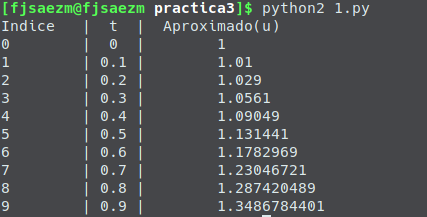
\includegraphics[scale=0.4]{1.png}
\end{center}

\section{Ejercicio 2 - Taylor de orden r}

\section{Ejercicio 5 - Runge-Kutta }
\begin{lstlisting}
  # -*- coding: utf-8 -*-
"""
    Estos serán los valores iniciales de nuestro programa:
    f(x,y) representa a la función de nuestro P.V.I
    [a,b] es el intervalo donde queremos aproximar
    n+1 serán los puntos de en los que aproximaremos.
"""

import math

def RungeKutta(f,a,b,n ,y_0):
    h=float(b-a)/n
    vals = []
    vals.append(y_0)
    valor=y(1)
    print ("Índice\t |  t  |  Aproximado(u) | Real(y) \t\t| Error")
    print ("0\t |  1  |"+str(y_0)+"\t|"+str(valor)+"  \t| "+str(valor-y_0))
    """
        NOTA: Ahora mismo los valores tj se machacan con cada interacción y los
        valores aproximados u se almacenan en el vector vals.
    """
    for i in range (0, n-1):
        tj =a+(i+1)*h
        Ki = []
        Ki.append(f(tj,vals[i]))
        Ki.append(f(tj+h/2,vals[i]+(h/2)*Ki[0]))
        Ki.append(f(tj+h/2,vals[i]+(h/2)*Ki[1]))
        Ki.append(f(tj+h,vals[i]+h*Ki[2]))
        x = vals[i] + (h/6)*(Ki[0]+2*Ki[1]+2*Ki[2]+Ki[3])
        valor=y(tj)
        vals.append(x)
        print (str(i+1)+"\t | "+str(tj)+" |"+str(x)+"\t|"+str(valor)+"  \t| "+str(valor-x))


def f(t,x):
    return math.pow(x,2)/(1+t);

def y(t):
    return -1/math.log(t+1)

"""En t=1"""
f0 = -1/(math.log(2))

RungeKutta(f,1,2,10,f0)
  \end{lstlisting}
\section{Ejercicio 7}
\begin{lstlisting}
  import numpy as num
import scipy as sci
from decimal import *
from numpy.polynomial import polynomial as pol

def pMedio(f,a,b,n,y_0):
    h=Decimal((b-a))/Decimal(n)
    vals = []
    vals.append(y_0)
    print ("Indice\t |  t  |  Aproximado(u) ")
    print ("0\t |  0  |\t"+str(y_0))
    vals.append(euler1(f,a,b,n,y_0))
    print ("1\t | "+ str(h) + " |\t"+str(vals[1]))
    for i in range (2, n):
        tj = a+(i*h)
        x = vals[i-2] + Decimal(2*h*f(tj,vals[i-1]))
        vals.append(x)
        print(str(i)+"\t | "+str(tj)+" |\t"+str(x))



def euler1(f,a,b,n,y_0):
    h=Decimal((b-a))/Decimal(n)
    tj = Decimal(a+h)
    x = y_0 + h*f(tj,y_0)
    return x

def y(t,x):
	return -x*t + math.pow(t,2)/2 + t

def f(t,x):
    return -x + t + 1

f0 = 1

pMedio(f,0,1,10,f0)
\end{lstlisting}
Si lo ejecutamos con la misma función y otros parámetros del ejercicio 1, obtenemos:
\begin{center}
  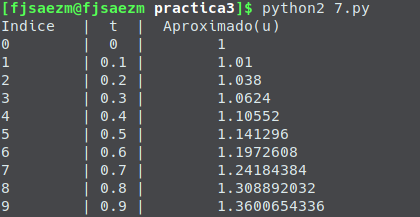
\includegraphics[scale=0.4]{7.png}
\end{center}

\section{Ejercicio 8}

\end{document}
